\section{Mathematische Grundlagen}

\begin{definition}[Torus]
Als \emph{Torus} bezeichnet man die Menge der Äquivalenzklassen definiert durch
\[
  \T \coloneqq \R / 2\pi\Z,
\]

gesprochen \enquote{$ \R $ modulo $ 2\pi\Z $}.
\end{definition}

\begin{remark}[Torus]
Einfach gesagt: Alle reellen Zahlen, die beim Teilen durch Vielfache von $ 2\pi $ den selben Rest 
lassen, sind äquivalent, und der Torus enthält alle möglichen Reste, die dabei auftreten können. 
Beispiel:
\[
0 / 2\pi = 0 \text{ Rest } 0, \quad 
2\pi / 2\pi = 1 \text{ Rest } 0, \quad 
4\pi / 2\pi = 2 \text{ Rest } 0, \dots
\]
D.h., die Zahlen $ 0 $, $ 2\pi $ und $ 4\pi $ sind zueinander äquivalent, da sie alle den Rest $ 0 $
lassen. Man sagt, sie befinden sich in einer gemeinsamen \emph{Äquivalenzklasse}. Da es unendlich
viele Zahlen gibt, die beim Teilen durch $ 2\pi $ den Rest $ 0 $ lassen, befinden sich unendlich
viele Zahlen in dieser Äquivalenzklasse. Daher sucht man sich einen Stellvertreter (einen sog.
\emph{Repräsentanten}), um vernünftig arbeiten zu können. Es bietet sich die einfachste Zahl in der
Äquivalenzklasse an, in diesem Fall die $ 0 $, und man schreibt dann häufig $ [0] $, wenn alle 
Zahlen gemeint sind, die zur $ 0 $ äquivalent sind.

Nun wird dem einen oder anderen schon aufgefallen sein, dass der Torus auch unendlich viele 
Äquivalenzklassen besitzt (da es ja unendlich viele mögliche Reste beim Teilen gibt).
Z.B.\ ist jede Zahl aus dem Intervall $ [0, 2\pi) $ ein Repräsentant genau einer Äquivalenzklasse,
und zu jeder Äquivalenzklasse kann man einen Repräsentanten in $ [0, 2\pi) $ finden. Daher sagt man
$ \T $ ist \emph{isomorph} zu $ [0, 2\pi) $, in Zeichen
\[
  \T \simeq [0, 2\pi).
\]
Wichtig: Das heißt \emph{nicht}, dass $ \T $ das Gleiche ist wie $ [0, 2\pi) $! $ [0, 2\pi) $
ist immer noch ein Intervall, und die Elemente aus $ \T $ können zwar mit denen aus $ [0, 2\pi) $ 
identifiziert werden, aber $ \T $ hat \emph{mehr Struktur} als $ [0, 2\pi) $. Denn: Wenn ich z.B. 
die Zahl $ \pi $ aus dem Torus mit sich selber addiere, dann bekomme ich $ 0 $, denn
$ \pi + \pi = 2\pi $ und $ 2\pi / 2\pi = 1 $ mit Rest $ 0 \in \T $. Das Ergebnis ist wieder ein 
Element aus dem Torus! Wenn ich aber $ \pi \in [0, 2\pi) $ betrachte, und die selbe Rechnung
wiederhole, dann bekomme ich immer noch $ 2\pi $. Aber im Unterschied zu vorher gilt jetzt
$ 2\pi \notin [0, 2\pi) $!

Übrigens gibt es unendlich viele Intervalle, die isomorph zu $ \T $ sind, z.B.
\[
  [-\pi, \pi), (-2\pi, 0], [-2\pi, 0), [42.5\pi, 44.5\pi), \dots
\]
Jedes Intervall der Länge $ 2\pi $ ist isomorph zu $ \T $! Aber man sucht sich natürlich nur die
hübschen Intervalle raus, und das sind im wesentlichen eh nur $ [0, 2\pi) $ und $ [-\pi, \pi) $.
\end{remark}

\begin{definition}[Funktionenräume] \leavevmode
\begin{enumerate}
\item Wir bezeichnen mit $ L(\R) $ die Gesamtheit aller reellwertigen Funktionen, d.h.\ die Menge 
  aller Funktionen, die von $ \R $ von $ \R $ abbilden:
  \[
    L(\R) = \{ f \colon \R \rightarrow \R \}.
  \]
  Analog ist $ l(\Z) $ die Menge aller reellwertigen Folgen, also Funktionen, die von $ \Z $ nach
  $ \R $ abbilden:
  \[
    l(\Z) = \{ c \colon \Z \rightarrow \R \}.
  \]
  Wichtig: Die Indexmenge der Folge kommt aus $ \Z $, das Bild einer Folge das aber 
  selbstverständlich weiterhin eine Teilmenge von $ \R $ sein. Wir könnten also auch schreiben:
  \[
    l(\Z) = \{ (c_{n})_{n \in \Z} \subseteq \R \}.
  \]
\item Die Menge aller summierbaren Funktionen $ L_{1}(\R) $ ist definiert durch
\[ 
  L_{1}(\R) \coloneqq \left\{
    f \in L(\R) \colon \norm{f}_{1} \coloneqq \int_{\R} |f(t)| \dif t < \infty
  \right\}
\]
und die Menge aller summierbaren Folgen durch
\[ 
  l_{1}(\Z) \coloneqq \left\{
    c \in l(\Z) \colon \norm{f}_{1} \coloneqq \sum_{k \in \Z} |c(k)| < \infty
  \right\}
\]
Bildlich Dargestellt kann man sich dies so vorstellen:
\begin{figure}[h]
\centering
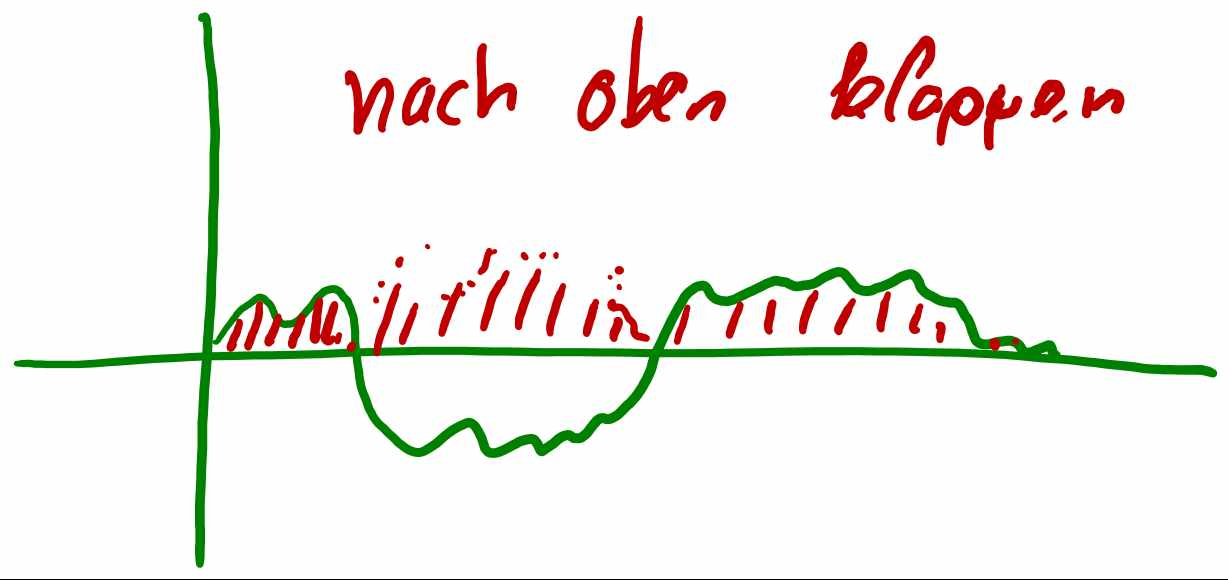
\includegraphics[width=0.5\linewidth]{Bilder/L1}
\caption{Hinreichend schnelles Abklingverhalten von $ L_{1}(\R) $-Funktionen.}
\label{fig:L1}
\end{figure}




\item Analog wird die Menge der quadratsummierbaren Funktionen $ L_{2}(\R) $ definiert durch
\[ 
  L_{2}(\R) \coloneqq \left\{
    f \in L(\R) \colon \norm{f}_{2} \coloneqq \sqrt{ \int_{\R} |f(t)|^{2} \dif t } < \infty
  \right\}
\]
und die Menge der quadratsummierbaren Folgen durch
\[ 
  l_{2}(\Z) \coloneqq \left\{
    c \in l(\Z) \colon \norm{c}_{2} \coloneqq \sqrt{ \sum_{k \in \Z} |c(k)|^{2} } < \infty.
  \right\}
\]
$ \norm{\bullet}_{2} $ bezeichnet man auch als die \enquote{Energie-Norm}.\\
Bildlich Dargestellt kann man sich dies so vorstellen:
\begin{figure}[h]
	\centering
	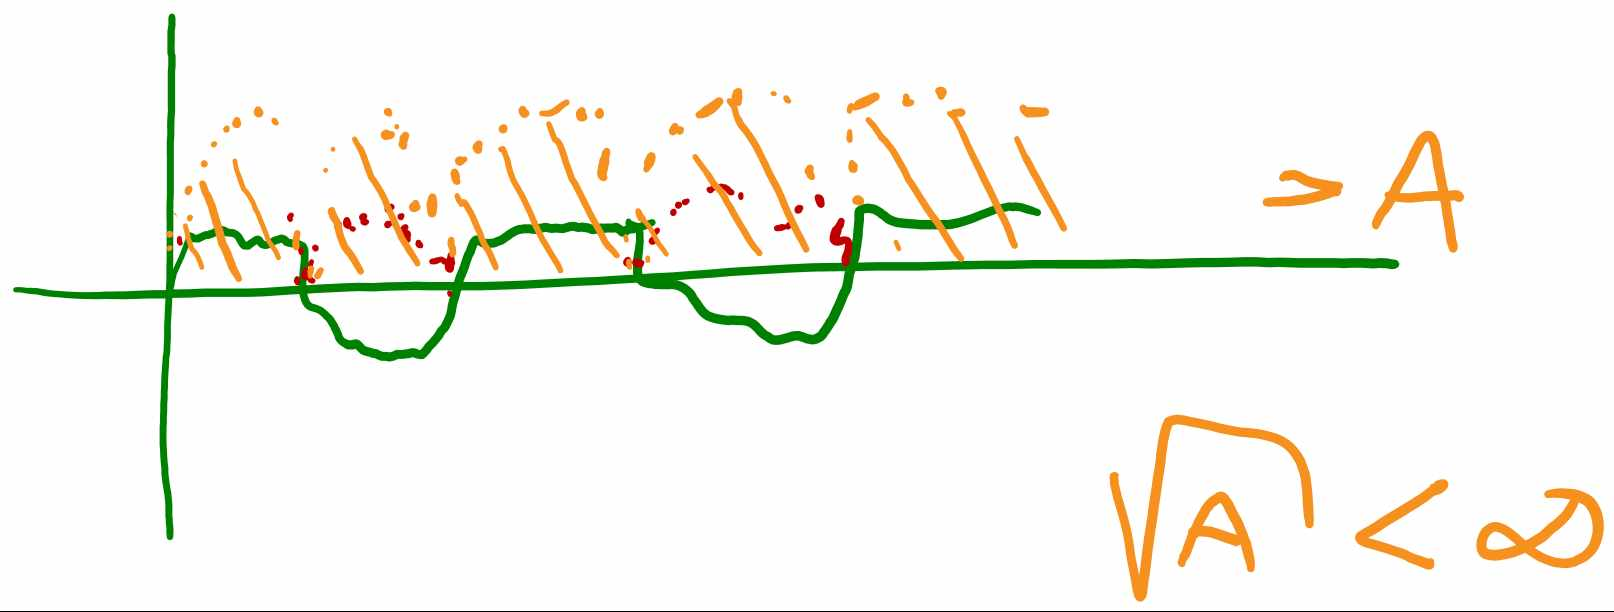
\includegraphics[width=0.5\linewidth]{Bilder/L2}
	\caption{Geometrische Interpretation als Mittelwert einer Fläche.}
	\label{fig:L2}
\end{figure}
\item Die Menge aller beschränkten Funktionen und Folgen definiert durch
\[
  L_{\infty}(\R) \coloneqq \left\{
    f \in L(\R) \colon \norm{f}_{\infty} \coloneqq
      \sup_{t \in \R} |f(t)| < \infty
  \right\}
\]
bzw.
\[
  l_{\infty}(\Z) \coloneqq \left\{
    c \in l(\Z) \colon \norm{c}_{\infty} \coloneqq
      \sup_{k \in \Z} |c(k)| < \infty
  \right\}.
\]
\item Einer geht noch: Die Menge der Funktionen und Folgen mit \emph{endlichem Träger}, geschrieben
als $ L_{00}(\R) $ bzw.\ $ l_{00}(\Z) $. Was ist mit \enquote{endlichem Träger} gemeint? Das 
bedeutet, dass der Bereich, auf dem die Funktion bzw.\ Folge lebt, nicht unendlich groß sein darf.
Formal: Es existiert ein $ N \in \N $, sodass
\[
  \left.
  \begin{array}{r}
    \{ t \in \R \colon f(t) \neq 0 \} \\
    \{ k \in \Z \colon c(k) \neq 0 \}
  \end{array}
  \right\}
  \subseteq [-N, N].
\]
\end{enumerate}
\end{definition}

\begin{remark}[$ L_{1}(\R) $-Funktionen und $ l_{1}(\Z) $-Folgen]
Wir betrachten nur Funktionen (bzw. Folgen, aber das werde ich jetzt nicht mehr dazu 
sagen), die \enquote{brav} sind. Damit ist gemeint, dass die Funktionen ein hinreichend schnelles 
Abklingverhalten gegen $ 0 $ besitzen müssen. Anschaulich gesprochen bewirkt der Betrag ja, dass 
wir einfach alles, was von der Funktion unterhalb der $ x $-Achse liegt, nach oben 
\enquote{umklappen}, sodass es nun positiv ist. Und wenn wir jetzt darüber integrieren, darf nur 
was Endliches dabei herauskommen. Dies ist eine hinreichende Forderung, damit wir die 
Fourier-Transformation zu einer Funktion überhaupt vernünftig definieren können.

Wir stellen fest, dass in $ l_{1}(\Z) $ \emph{nur} Nullfolgen (Folgen, deren
Grenzwert $ 0 $ ist) zu finden sind, z.B.\ $ (1 / k^2)_{k \in \Z} $. Achtung! Die Folge 
$ (1 / k)_{k \in \Z} $ ist zwar auch eine Nullfolge, aber die Reihe dazu konvergiert nicht 
absolut (wir haben es hier ja mit der harmonischen Reihe zu tun), und ist daher ist die Folge auch 
nicht in $ l_{1}(\Z) $.
\end{remark}

\begin{remark}[$ L_{2}(\R) $-Funktionen und $ l_{2}(\Z) $-Folgen]
Unterschied zu den \enquote{normalen} summierbaren Funktionen ist, dass hier die Zwei-Norm der
Funktion kleiner als unendlich sein muss anstatt der Eins-Norm (daher kommt ja auch der Name
\enquote{quadratsummeribar}). Leider gibt es hierfür keine so schöne geometrische Anschauung, da wir
über ganz $ \R $ integrieren, aber man kann versuchen, sich das Ganze so vorzustellen: Durch das
Quadrieren des Betrags erhält man sozusagen eine Fläche, und durch das Integrieren erzeugen wir
ein Volumen, welches dann so wie ein Schlauch an der $ x $-Achse entlang wabert. Durch das 
Wurzelziehen brechen wir das Volumen wieder herunter auf eine Fläche. Und hier endet leider schon
die Analogie. Auf dem Torus würde man jetzt noch durch $ 2\pi $ teilen (weil das die Länge eines
Intervalls ist, welches isomorph zum Torus ist), und man könnte sich die Zwei-Norm vorstellen als
Mittelwert der Fläche. Da wir aber über ganz $ \R $ integrieren und wir schlecht durch $ \infty $
teilen können, lass ma das hier bleiben und geben uns mit dem zufrieden, was wir schon haben. 

Das führt uns unweigerlich zu einer wichtigen Frage: Warum sollte man also überhaupt den Raum $ 
L_{2}(\R) $ definieren wollen? Die Antwort ist: Weil Mathematiker es immer cool finden, 
irgendwelche abgefahrenen Konzepte zu verallgemeinern. Außerdem kann man in $ L_{2}(\R) $ ein 
Skalarprodukt von Funktionen definieren, mit dem sich recht schön rechnen lässt, was eben in 
$ L_{1}(\R) $ nicht geht.

Für die mathematisch Interessieren unter uns: $ L_{2}(\R) $ liegt dicht in $ L_{1}(\R) $, und es
gilt:
\[
  L_{1}(\R) \nsubset L_{2}(\R) \quad \text{und} \quad L_{2}(\R) \nsubset L_{1}(\R).
\]
Cool ist es aber, wenn wir Funktionen im Schnitt der beiden Funktionenräume betrachten. Für solche
Funktionen kann man nämlich wieder eine Fourier-Transformierte definieren, und man hat sogar ein
Skalarprodukt.
\end{remark}

\begin{example}[Beschränkte Folge]
Betrachten wir als Beispiel einer Folge in $ l_{\infty}(\Z) $ die Folge $ ((-1)^{n} : n \in \Z) $.
Die Folge besitzt zwei Häufungspunkte $ -1 $ und $ 1 $, zwischen denen sie immer hin- und 
herspringt. Das Supremum dieser Folge ist natürlich $ 1 $, was kleiner als $ \infty $ ist. Wäre 
diese Folge auch in $ l_{1}(\Z) $? Nein, wäre sie nicht, da sie ja nicht mal konvergiert.
\end{example}

\begin{example}[$ L_{00}(\R) $-Funktion]
Die Exponentialfunktion $ \exp $ wird niemals $ 0 $, sie hat unendlichen Träger und
deshalb keine $ L_{00}(\R) $-Funktion. Die Rechtecksfunktion $ \chi_{[-1,1]} $ hingegen ist nur
im Intervall $ [-1,1] $ ungleich $ 0 $ und daher in $ L_{00}(\R) $.
\end{example}

\begin{definition}[Dirac-Puls]
Der Dirac-Puls
\[
  \delta(k) \coloneqq \delta_{0k} \coloneqq 
  \begin{cases}
    1,& k = 0, \\ 0,& k \neq 0
  \end{cases}
\]
ist eine lustige Funktion, die nur an der Stelle $ 0 $ gleich $ 1 $ ist und sonst überall $ 0 $
(siehe Abbildung~\ref{fig:dirac}).
\begin{figure}[ht]
\centering
\begin{tikzpicture}
\draw [->] (-4.5,0) -- (4.5,0) node [right] {$ x $};
\foreach \x in {-4,-3,...,4}{
  \draw (\x, -0.1) node [below] {$ \x $} -- (\x, 0.1);
}
\draw [->] (0,0) -- (0,1) node [right] {$ 1 $} -- (0,1.5) node [right] {$ \delta(x) $};
\draw (-0.1,1) -- (0.1,1);
\draw [color=red, thick] (0,0) -- (0,1);
\end{tikzpicture}
\label{fig:dirac}
\caption{Der Dirac-Puls $ \delta $.}
\end{figure}
\end{definition}

\begin{definition}[Abtastoperator]
Der Abtastoperator $  S_{h} : L(\R) \rightarrow l(\R) $ mit Schrittweite $ h $ ist für eine
Funktion $ f $ definiert als
\[
  (S_{h}f)(k) \coloneqq f(hk), \quad k \in \Z.
\]
\end{definition}

\begin{remark}[Abtastoperator]
Anstatt die Funktion für alle reellen Zahlen zu betrachten, tasten wir die Funktion
nur an abzählbar vielen Stellen im Abstand $ h \in \R $ ab. Wir betrachten
die Funktion also nur an den Stellen $ 0, h, -h, 2h, -2h, 3h, -3h \dots $, was effektiv zu einer
Diskretisierung des gegebene kontinuierlichen Signals führt. Dieses Prozess kann man auch als
\emph{Downsampling} bezeichnen.
\end{remark}

\begin{figure}[ht]
\centering
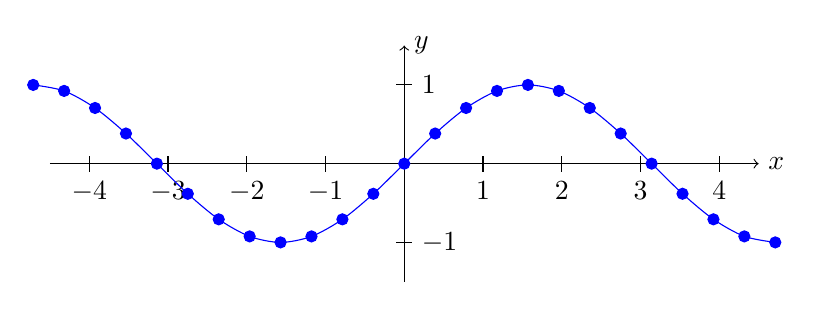
\begin{tikzpicture}
\draw [->] (-4.5,0) -- (4.5,0) node [right] {$ x $};
\draw [->] (0,-1.5) -- (0,1.5) node [right] {$ y $};
\foreach \x in {-4,-3,-2,-1,1,2,3,4}{
  \draw (\x,-0.1) node [below] {$ \x $} -- (\x,0.1);
}
\foreach \y in {-1,1}{
  \draw (-0.1,\y) -- (0.1,\y) node [right] {$ \y $};
}
\draw [color=blue, mark=*,] plot [domain=-1.5*pi:1.5*pi,smooth] (\x,{sin(deg(\x))});
\end{tikzpicture}
\label{fig:abtastoperator}
\caption{Abtastung des sinus an den hervorgehobenen Punkten.}
\end{figure}